\documentclass{../../zirkelblatt1718}
\graphicspath{{../}}
\usepackage{multicol,mathtools,booktabs,xspace,wrapfig}
\usepackage{tikz}
\usetikzlibrary{arrows,decorations.pathreplacing}
\usepackage{subfig}

\theoremstyle{definition}
\newtheorem{defn}{Definition}
\newtheorem{bsp}[defn]{Beispiel}

\theoremstyle{plain}
\newtheorem{prop}[defn]{Proposition}
\newtheorem{satz}[defn]{Satz}
\newtheorem{lemma}[defn]{Lemma}

\theoremstyle{remark}
\newtheorem{bem}[defn]{Bemerkung}
\newtheorem{aufg}[defn]{Aufgabe}
\newtheorem{tipp}[defn]{Tipp}
\newtheorem{motto}[defn]{Motto}

\renewcommand{\NN}{\mathbb{N}}
\newcommand{\RR}{\mathbb{R}}
\newcommand{\Slope}{S}
\newcommand{\Front}{F}
\newcommand{\Intersect}{\Delta}

\newcommand{\defeq}{\vcentcolon=}

\newcommand{\happy}{
\includegraphics[height=0.7em]{happy}\xspace}

\begin{document}

\maketitleCustom{Klassen 11/12}{\textbf{\textsf{%
  Große Zahlen \\
  \normalsize Korrespondenzzirkel vom 4. April 2018}}}

Ahoi! Mit diesem Brief möchten wir Neugierde an etwas ganz Alltäglichem wecken:
natürlichen Zahlen. Wir möchten euch allerlei Sorten von Zahlen vorstellen:

\begin{enumerate}
\item Zahlen, von denen man genau weiß, dass sie höchstens zwei Stellen haben,
aber die Bestimmung ihres exakten Werts noch völlig außerhalb unserer
Möglichkeiten steht.
\item Zahlen, die absurd groß sind: So groß, dass es nicht genügend Atome im
sichtbaren Universum gibt, um sie jemals aufzuschreiben -- ja sogar so groß,
dass es nicht genügend Atome gibt, um die Anzahl ihrer Stellen zu verewigen --
sogar so groß, dass es nicht genügend Atome gibt, um die Anzahl der Stellen der
Anzahl der Stellen niederzuschreiben -- ja sogar so groß \ldots{} Das geht noch
eine lange Zeit so weiter (wie lange, können wir nicht aufschreiben).
\item Zahlenfolgen, die so schnell anwachsen, dass sie selbst im Prinzip nicht
berechenbar sind -- die absurd großen Zahlen aus dem letzten Absatz können zwar
schon nicht in unserem physischen Universum berechnet werden, aber die Zahlenfolgen
an die wir jetzt denken setzen noch einen drauf: Bewiesenermaßen könnten sie
auch nicht in einem hypothetischen größeren Universum berechnet werden. Bei
denen ist es \emph{mathematisch unmöglich}, ihren Zahlenwert algorithmisch zu
bestimmen, und weder Unmengen an Speicherplatz und Energie noch Intelligenz
kann daran etwas ändern.
\end{enumerate}

Dabei geht es uns stets primär um \emph{endliche Zahlen}. Nur die gehören
konventionsgemäß zu der Menge der natürlichen Zahlen. In der Mathematik werden
aber auch \emph{unendlich große Zahlen} untersucht, welche zum einen für sich
selbst interessant sind und uns zum anderen zur Konstruktion absurd großer
endlicher Zahlen helfen werden. Hier ein Vorgeschmack auf den \emph{ordinalen
Zahlenstrahl}, der auch unendlich große Zahlen umfasst:
\[ 0, 1, 2, \ldots, \omega, \omega + 1, \omega + 2, \ldots,
  \omega\cdot2, \ldots\ldots, \omega\cdot3, \ldots\ldots\ldots, \omega^2,
  \ldots\ldots\ldots\ldots, \omega^3
  \]
Und ja, es gibt sogar Ungetüme wie
\[ \varepsilon_0 = \omega^{\omega^{\omega^{\omega^{\ldots}}}}, \]
etwas schwammig ausgesprochen "`unendlich hoch unendlich hoch unendlich hoch
\ldots, insgesamt unendlich oft"'. Spoiler: Gestandene Mengentheoretikerinnen
lächeln nur müde über~$\varepsilon_0$; in ihrer Forschung beschäftigen sie sich
mit weit größeren Zahlen. Aber alles zu seiner Zeit.

Wenn du diese Figur siehst:
\begin{center}
\includegraphics[width=0.1\textwidth]{happy}\end{center}
Dann halte beim Lesen kurz inne und überzeuge dich von der Behauptung, um die
es gerade geht. Oder lies erst mal weiter, ganz wie du magst. Aber wir laden
dich herzlich ein, über diesen Stellen zu grübeln -- sie machen Spaß! Wenn du
nicht siehst, wie man eine solche Stelle genauer begründet, dann schreib uns
einfach. Die Illustration haben wir übrigens von SpikedMath.com übernommen,
einem nerdigen Comic.


\section{Kleine Zahlen, deren exakter Wert uns noch lange verschlossen bleiben wird}

\subsection{Einstieg in die Partymathematik}

\begin{prop}
Auf jeder Party mit mindestens sechs Gästen gibt es stets mindestens drei
Gäste, die sich vorher schon alle untereinander kannten, oder drei Gäste, die
sich vorher alle untereinander nicht kannten.
\end{prop}

Lasst uns dieses Kuriosum beweisen!

\begin{proof}Wir betrachten eine beliebige Party mit mindestens sechs Gästen
und möchten unser Augenmerk auf einen der Gäste, Gast~$A$, richten. Es gibt
entweder
\begin{enumerate}
\item noch mindestens drei Leute, Gäste~$B$, $C$ und~$D$, sodass sich~$A$--$B$,
$A$--$C$ und~$A$--$D$ schon vorher kannten; oder
\item es gibt mindestens drei Leute, Gäste~$B$, $C$ und~$D$, sodass
sich~$A$--$B$, $A$--$C$ und~$A$--$D$ vorher nicht kannten. (Oder beides.)
\end{enumerate}
Überzeuge dich davon!~\happy An dieser Stelle geht ein, dass es insgesamt mindestens
sechs Gäste gibt. Lasst uns die beiden Fälle separat untersuchen:

In Fall~a) könnte es sein, dass sich~$B$--$C$,~$B$--$D$ oder~$C$--$D$ schon kannten.
Dann bilden die drei Gäste~$A$--$B$--$C$ bzw.~$A$--$B$--$D$ bzw.~$A$--$C$--$D$
ein Dreiergrüppchen, das sich schon vorher kannte. Es kann aber auch sein, dass
sich~$B$--$C$,~$B$--$D$ oder~$C$--$D$ alle nicht kannten. Dann
bilden~$B$--$C$--$D$ ein Dreiergrüppchen, das sich vorher nicht kannte. So oder
so stimmt die Behauptung des Theorems.

In Fall~b) verhält es sich ähnlich. (Wie genau? \happy)
\end{proof}


\subsection{Ramsey-Theorie}

Die Proposition zur Partymathematik illustriert den \emph{Hauptsatz der
Ramsey-Theorie}, einem großen Teilgebiet der Kombinatorik. Er besagt:

\begin{satz}Zu jeder natürlichen Zahl~$r$ und jeder natürlichen Zahl~$b$ gibt
es eine natürliche Zahl~$N$ mit folgender Eigenschaft: In jeder Party mit
mindestens~$N$ Gästen gibt es ein Grüppchen aus~$r$ Gästen, die sich alle schon
vorher kannten, oder ein Grüppchen aus~$b$ Gästen, die sich alle vorher noch
nicht kannten.
\end{satz}

Die eben bewiesene Proposition ist ein Spezialfall dieses Satzes, nämlich für
den Fall~$r = 3$ und~$b = 3$. Wenn man den Satz auf Wikipedia nachschlägt, ist
nicht von Partys, sondern von \emph{Graphen} die Rede, und es geht nicht darum,
ob sich Gäste schon kannten, sondern darum, ob Kanten zwischen je zwei Knoten
rot oder blau gefärbt sind (so erklären sich auch die Variablennamen). Es
können auch beide Fälle eintreten; wenn man in der Mathematik das Wort "`oder"'
verwendet, meint man damit nicht, dass \emph{genau} einer der beiden Fälle
eintritt.

Es ist mühsam, immer von Leuten, die sich schon kannten, oder Leuten, die sich
noch nicht kannten, zu sprechen. Lasst uns ab jetzt folgende Sprechweise
übernehmen: Grüppchen aus Leuten, die sich schon kannten, heißen \emph{rote
Grüppchen}, und Grüppchen aus Leuten, die sich noch nicht kannten, heißen
\emph{blaue Grüppchen}. Statt "`Grüppchen bestehend aus~$k$~Leuten"' wollen
wir auch kurz~"`$k$-Grüppchen"' schreiben.

Vor vornherein ist es überhaupt nicht einsichtig, wieso der Satz stimmen
sollte, wieso es also in Abhängigkeit von~$r$ und~$b$ eine Anzahl~$N$ geben
sollte, sodass es in \emph{jeder} Party mit~$N$ Gästen mit ihren irgendwie
gearteten Bekanntheitsbeziehungen stets ein rotes~$r$-Grüppchen oder ein
blaues~$b$-Grüppchen geben sollte. Dass der Satz trotzdem stimmt, zeigt sein
Beweis, den wir weiter unten präsentieren.

Die kleinstmögliche Zahl~$N$ mit den genannten Eigenschaften schreibt man auch
als~"`$R(r,g)$"'. Die Eingangsproposition kann man also in folgende Sprache
kleiden: Die Zahl~$R(3,3)$ ist höchstens sechs.~\happy Man kann sich nun zusätzlich
überlegen, dass es bei nur fünf Gästen mindestens eine Gästekonstellation gibt,
in der weder ein Dreiergrüppchen aus Leuten, die sich schon kannten, noch ein
Dreiergrüppchen aus Leuten, die sich noch nicht kannten, gibt.~\happy Daher
ist~$R(3,3)$ genau gleich sechs.


\subsection{Unser Wissensstand}

Wie kann man die \emph{Ramsey-Zahlen}~$R(r,g)$ bestimmen? Prinzipiell ist das
leicht, man muss nur einen Computer beauftragen, alle möglichen
Gästekonstellationen durchzugehen und dabei zu prüfen, ab welcher Partygröße es
immer mindestens ein rotes~$r$-Grüppchen oder ein blaues~$b$-Grüppchen gibt.
Allerdings gibt es unzählige solcher Konstellationen,\footnote{Lasst uns grob
überschlagen, wie viele verschiedene Gästekonstellationen es bei insgesamt zehn
Gästen gibt. Es gibt~$\binom{10}{2} = 10 \cdot 9 / 2 = 45$ viele Paare von je zwei
Gästen. Also gibt es~$2^{45}$ Möglichkeiten für die "`kannten sich
schon"'/"`kannten sich noch nicht"'-Optionen, die es für jedes Paar gibt. Das
sind etwa 35~Trillionen. Die tatsächlich relevante Anzahl Möglichkeiten ist
etwas geringer, da es auf die Reihenfolge der Personen nicht ankommt.}
und es sind nur wenige Abkürzungen bekannt, die es dem Computer ermöglichen,
ein paar Fälle nicht überprüfen zu müssen. Deswegen sind die meisten
Ramsey-Zahlen unbekannt.

Bis 2012 wusste man von~$R(4,6)$ etwa nur, dass diese Zahl zwischen~35 und~41
liegt (jeweils einschließlich). Seit einem neuen Ergebnis im Jahr 2012 weiß
man: Die Zahl~$R(4,6)$ liegt zwischen~\emph{36} und~41 (jeweils
einschließlich). Diese Erkenntnis war einen mathematischen Fachartikel
wert.\footnote{Interessiert? Eine Suchmaschine wird ihn auftreiben: \emph{On
the Ramsey Number~$R(4,6)$} von Geoffrey Exoo, The Electronic Journal of
Combinatorics, 2012.}

Überlege dir, wie man grundsätzlich vorgehen muss, um \emph{untere Schranken}
für die Ramsey-Zahlen zu finden -- also herauszufinden, dass eine bestimmte
Ramsey-Zahl mindestens so und so groß ist.~\happy Wie man vorgehen kann, um
(nicht optimale, aber immerhin irgendwelche) \emph{obere} Schranken zu finden,
behandeln wir im nächsten Abschnitt.


\subsection{Obere Schranken}

Unendlich viele Ramsey-Zahlen sind heute unbekannt, aber unendlich viele andere
lassen sich leicht bestimmen: Überzeuge dich davon, dass für alle positiven
natürlichen Zahlen~$r$ und~$b$ gilt: $R(r,1) = 1$ und~$R(1,b) = 1$.~\happy (Was
bedeutet das? Hat was mit etwas einsamen \emph{Einergrüppchen} zu tun.)

Nächstschwieriger sind folgende Erkenntnisse:

\begin{itemize}
\item Für alle natürlichen Zahlen~$r$ gilt $R(r,2) = r$.~\happy
\item Für alle natürlichen Zahlen~$b$ gilt $R(2,b) = b$.~\happy
\item Für alle natürlichen Zahlen~$r$ und~$b$ gilt: $R(r,b) = R(b,r)$.~\happy
\end{itemize}

Mit solchen Erkenntnissen setzt man folgende allgemeine Beobachtung in Gang, die
dann den Hauptsatz der Ramsey-Theorie beweist. Nimm dir Zeit, die Formulierung
des Lemmas und den Beweis zu verstehen!~\happy

\begin{lemma}Seien~$r$ und~$b$ beliebige natürliche Zahlen. Sei schon bekannt,
dass es Zahlen~$P$ und~$Q$ mit folgenden Eigenschaften gibt:
\begin{itemize}
\item Auf jeder Party mit~$P$ Gästen gibt es mindestens ein
rotes~$(r-1)$-Grüppchen oder mindestens ein blaues~$b$-Grüppchen.
(Kurz: $R(r-1,b) \leq P$.)
\item Auf jeder Party mit~$Q$ Gästen gibt es mindestens ein
rotes~$r$-Grüppchen oder mindestens ein blaues~$(b-1)$-Grüppchen.
(Kurz: $R(r,b-1) \leq Q$.)
\end{itemize}
Dann gibt es auf jeder Party mit mindestens~$P+Q$ Gästen mindestens ein
rotes~$r$-Grüppchen oder mindestens ein blaues~$b$-Grüppchen. (Kurz: Die
Zahl~$R(r,b)$ gibt es wirklich, und zwar gilt~$R(r,b) \leq P + Q$.)
\end{lemma}

\begin{proof}Wir betrachten eine beliebige Gästekonstellation mit insgesamt
mindestens~$P + Q$ Gästen und richten unser Augenmerk auf einen der Gäste,
Gast~$A$. Wir müssen beweisen, dass es mindestens ein rotes~$r$-Grüppchen oder
mindestens ein blaues~$b$-Grüppchen gibt.

Sei~$M$ die Menge derjenigen restlichen Gäste, die~$A$ schon vorher
kannten (und die~$A$ vorher schon kannte), und~$N$ die Menge derjenigen
restlichen Gäste, die~$A$ vorher noch nicht kannten (und die~$A$ auch vorher
noch nicht kannte).

Nun folgt, dass a) zu~$M$ mindestens~$P$ Gäste gehören oder b) dass zu~$N$
mindestens~$Q$ Gäste gehören. Denn angenommen, zu~$M$ würden höchstens~$P-1$
und zu~$N$ würden höchstens~$Q-1$ Gäste gehören: Dann gäbe es auf der Party
insgesamt nur~$1 + (P-1) + (Q-1) = P+Q-1$ Gäste. Es gibt ja aber
mindestens~$P+Q$ Gäste.~\happy

Jeden der beiden Fälle untersuchen wir nun separat.

\begin{enumerate}
\item Nach Voraussetzung an~$P$ gibt es unter den zu~$M$ gehörenden Gästen
mindestens ein rotes~$(r-1)$-Grüppchen~$G$ oder mindestens ein
blaues~$b$-Grüppchen. Falls letzteres, sind wir mit unserem Beweis
fertig (wieso?~\happy). Falls ersteres, dann sind wir ebenfalls fertig, da
das~$r$-Grüppchen bestehend aus den Gästen in~$G$ und zudem Gast~$A$ rot
ist.~\happy
\item Wenn du die Überlegung zu Fall~a) verstanden hast, dann versuche, die
Überlegung zu Fall~b) selbstständig zu führen!~\happy \qedhere
\end{enumerate}
\end{proof}

Kurz zusammengefasst besagt das Lemma, dass
\[ R(r,b) \leq R(r-1,b) + R(r,b-1), \]
und mit dieser Abschätzung kann man für jede Ramsey-Zahl obere Schranken
angeben. Wenn wir zum Beispiel noch nicht wüssten, dass~$R(3,2) = 3$ ist,
könnten wir uns diesem Resultat wie folgt nähern:
\[ R(3,2) \leq R(2,2) + R(3,1) \leq R(1,2) + R(2,1) + R(3,1) =
  1 + 1 + 1 = 3. \]
Wir können etwa auch folgern:
\[ R(4,3) \leq R(3,3) + R(4,2) = 6 + 4 = 10. \]
(Tatsächlich gilt~$R(4,3) = 9$, die obere Schranke ist hier also sehr nah am
tatsächlichen Wert.)
Und weiter:
\[ R(4,4) \leq R(3,4) + R(4,3) = R(4,3) + R(3,4) \leq 10 + 10 = 20. \]
(Der tatsächliche Wert von~$R(4,4)$ ist~$18$.)

Wenn du Spaß am Programmieren hast, oder es lernen möchtest, dann schreibe doch
ein Programm, dass nach diesem Schema obere Schranken für die Ramsey-Zahlen
ausgibt.~\happy


\section{Sehr große Zahlen}

\subsection{Hyperoperationen}

Addition, Multiplikation, Exponentiation -- wie geht es weiter? Mit der
\emph{Tetration}!
\begin{align*}
  2 \cdot 5 &= 2 + 2 + 2 + 2 + 2 \\
  2 \uparrow 5 &= 2^5 = 2 \cdot 2 \cdot 2 \cdot 2 \cdot 2 \\
  2 \uparrow\uparrow 5 &= 2^{2^{2^{2^{2}}}} \quad
  \text{(eine Zahl mit 19729 Stellen)}
\end{align*}
Der Potenzturm könnte missverständlich sein -- ist
$2^{(2^{(2^{(2^2)})})}$ oder ist~${\Bigl({\bigl({(2^2)}^2\bigr)}^2\Bigr)}^2$ gemeint?
Man hat sich dazu entschieden, die erste Möglichkeit zu meinen, denn die andere
Möglichkeit könnte man noch vereinfachen (wozu?~\happy). Übrigens liefert die
erste Möglichkeit auch den größeren Zahlenwert (wieso?~\happy).

Jedenfalls: Wieso bei zwei Pfeilen aufhören? Nach der Tetration kommt \ldots
\[
  2 \uparrow\uparrow\uparrow 5 =
  2 \uparrow\uparrow 2 \uparrow\uparrow 2 \uparrow\uparrow 2 \uparrow\uparrow 2
\]
Auch hier sollte man wieder präzisieren, was gemeint ist: nämlich die Zahl~$2
\uparrow\uparrow (2 \uparrow\uparrow (2 \uparrow\uparrow (2 \uparrow\uparrow
2)))$, nicht die Zahl~$(((2 \uparrow\uparrow 2) \uparrow\uparrow 2)
\uparrow\uparrow 2) \uparrow\uparrow 2$. Die Zahl~$2 \uparrow\uparrow\uparrow
5$ ist ein gewaltiger Potenzturm aus Zweiern -- genauer gesagt: einer aus~$2
\uparrow\uparrow (2 \uparrow\uparrow (2 \uparrow\uparrow 2))$ vielen Zweien.
Die Anzahl dieser Zweien ist also selbst ein riesiger Potenzturm -- einer
aus~$2 \uparrow\uparrow (2 \uparrow\uparrow 2) = 65536$ Zweien.

Diese Rechenoperationen -- und die weiteren, die man analog definieren kann,
wie etwa~$\uparrow\uparrow\uparrow\uparrow$ -- heißen auch
\emph{Hyperoperationen}. Hier ein paar Aufgaben zum Vertrautwerden:

\begin{itemize}
  \item Welche der Zahlen~$2 \uparrow\uparrow (2 \uparrow\uparrow 2)$ und~$(2
  \uparrow\uparrow 2) \uparrow\uparrow 2$ ist größer?~\happy
  \item Wieso ist~$2 \uparrow\uparrow\uparrow\uparrow\uparrow 2 = 4$?~\happy
  \item Wieso ist~$2 \uparrow\uparrow\uparrow\uparrow\uparrow 1 = 2$?~\happy
\end{itemize}


\subsection{Grahams Zahl}

\begin{wrapfigure}{r}{0.2\textwidth}
\vspace*{-1em}
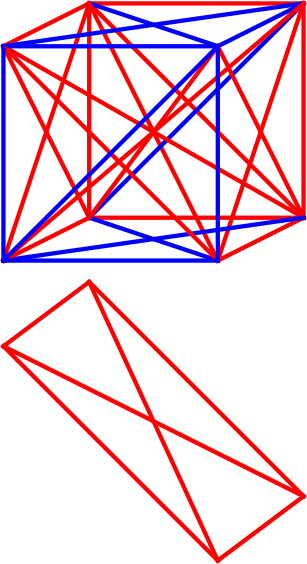
\includegraphics[width=0.2\textwidth]{graham}
\end{wrapfigure}

Mit den Hyperoperationen ausgerüstet, können wir uns ans Werk machen, um
\emph{Grahams Zahl} zu definieren -- eine Zahl, die auf eine kombinatorische
Untersuchung von Ronald Graham zurückgeht und für eine Weile den Titel
beanspruchte, die größte natürliche Zahl zu sein, die jemals in einem
mathematischen Beweis explizit verwendet wurde.

Graham fragte sich: Stimmt es eigentlich, dass es, egal mit welchen zwei Farben
man die~28~Kanten des dreidimensionalen Würfels einfärbt (Flächen- und
Raumdiagonalen dazugezählt), stets mindestens vier Eckpunkte gibt, die in einer
gemeinsamen Ebene liegen und deren Verbindungen alle dieselbe Farbe haben?

Das ist etwa bei der Färbung in der oberen Skizze der Fall. Allerdings würde es
keine solchen vier Eckpunkte geben, wenn die von unten vorne rechts nach unten
hinten rechts verlaufende Kante blau eingefärbt wäre. Die Antwort auf Grahams
Frage lautet daher: Nein, das stimmt nicht immer.

Das war auch Graham schnell klar, und so stellte er die analoge Frage für den
vierdimensionalen Würfel mit seinen 16~Ecken und 135~Querverbindungen. Aber
auch bei ihm gibt es eine Färbung, sodass kein Satz aus vier in einer
gemeinsamen Ebene liegenden Eckpunkten mit lauter gleichfarbigen
Querverbindungen existiert.

\begin{center}
  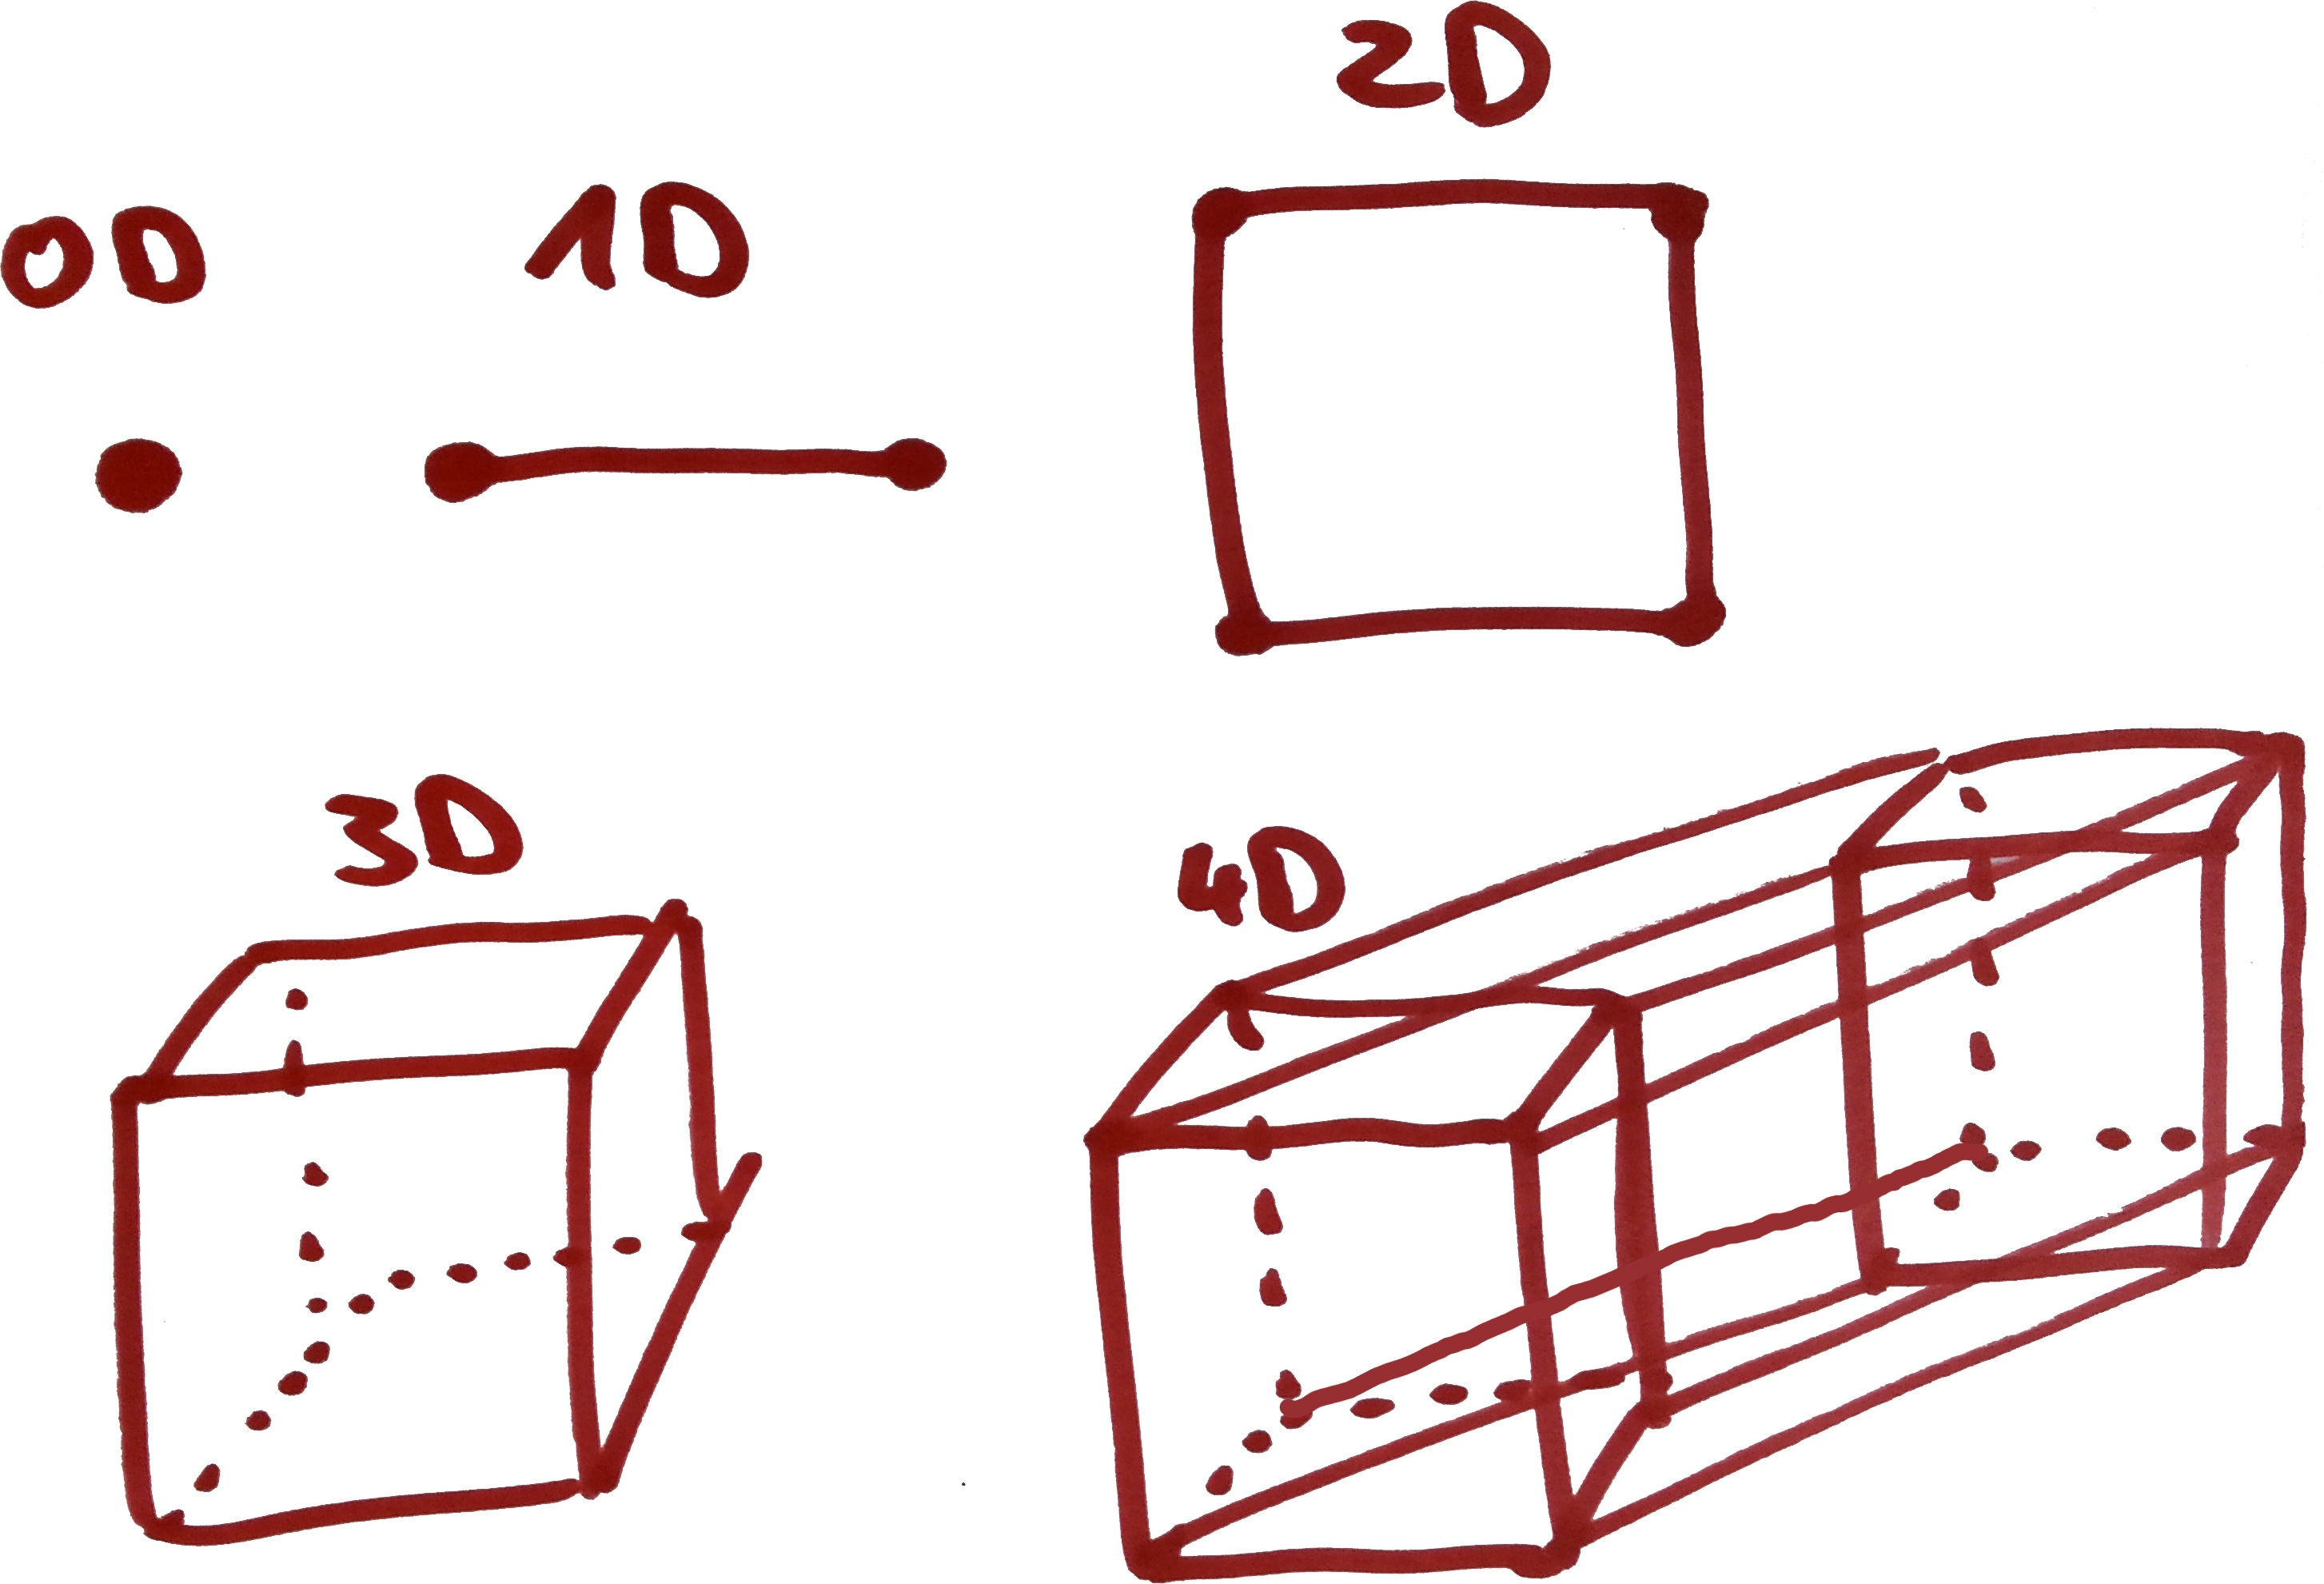
\includegraphics[width=0.7\textwidth]{4d-tesseract}
\end{center}

Beim fünf-, sechs-, \ldots, dreizehndimensionalen Würfel ist das genauso. Für
den vierzehndimensionalen Würfel ist die Frage offen. Graham zeigte: Zumindest
wenn man den~$G$-dimensionalen Würfel nimmt, dann stimmt es -- dann gibt es
immer mindestens vier Eckpunkte gibt, die in einer gemeinsamen Ebene liegen und
deren Querverbindungen alle dieselbe Farbe haben. Die Zahl~$G$ ist die
\emph{Grahamsche Zahl}. Sie ist wie folgt definiert:
\[
\left.
 \begin{matrix}
  G &=&3\underbrace{\uparrow \uparrow \cdots\cdots\cdots\cdots\cdots \uparrow}3 \\
    & &3\underbrace{\uparrow \uparrow \cdots\cdots\cdots\cdots \uparrow}3 \\
    & &\underbrace{\qquad\;\; \vdots \qquad\;\;} \\
    & &3\underbrace{\uparrow \uparrow \cdots\cdot\cdot \uparrow}3 \\
    & &3\uparrow \uparrow \uparrow \uparrow3
 \end{matrix}
\right \} \text{64 Schichten}
\]
In Worten: Man beginnt mit der Zahl~$g_1 = 3\uparrow \uparrow \uparrow \uparrow3$.
Dann nimmt man~$g_2 = 3 \uparrow \uparrow \ldots \uparrow \uparrow 3$ mit
insgesamt~$g_1$ vielen Pfeilen. Dann folgt~$g_3 = 3 \uparrow \uparrow \ldots
\uparrow \uparrow 3$ mit insgesamt~$g_2$ vielen Pfeilen. Und so macht man noch
eine ganz Zeit lang weiter, bis man bei~$g_{64}$ angekommen ist. Das ist
Grahams Zahl.~\happy

Zu Grahams Zahl ist noch viel, viel mehr zu berichten; wir sind uns aber nicht
sicher, was euch interessiert. Deswegen hören wir an dieser Stelle auf und
bitten euch, uns zu schreiben:

\begin{itemize}
  \item Interessiert ihr euch für vierdimensionale Geometrie? Möchtet ihr mehr
  über den vierdimensionalen Würfel erfahren? Möchtet ihr wissen, wie die
  Zahlenfolge~$1, \infty, 5, 6$ weiter geht?
  \item Die erste Ziffer von Grahams Zahl ist unbekannt. Die letzten Ziffern
  kann man aber recht einfach berechnen. Möchtet ihr wissen, wie das geht?
\begin{center}
\emph{Die letzten 500 Ziffern von Grahams Zahl:}

02425950695064738395657479136519351798334535362521 \\
43003540126026771622672160419810652263169355188780 \\
38814483140652526168785095552646051071172000997092 \\
91249544378887496062882911725063001303622934916080 \\
25459461494578871427832350829242102091825896753560 \\
43086993801689249889268099510169055919951195027887 \\
17830837018340236474548882222161573228010132974509 \\
27344594504343300901096928025352751833289884461508 \\
94042482650181938515625357963996189939679054966380 \\
03222348723967018485186439059104575627262464195387
\par
\end{center}
\end{itemize}

\end{document}
